\documentclass[letterpaper,12pt]{article}

\usepackage{threeparttable}
\usepackage{geometry}
\geometry{letterpaper,tmargin=1in,bmargin=1in,lmargin=1.25in,rmargin=1.25in}
\usepackage[format=hang,font=normalsize,labelfont=bf]{caption}
\usepackage{amsmath}
\usepackage{multirow}
\usepackage{array}
\usepackage{delarray}
\usepackage{amssymb}
\usepackage{amsthm}
\usepackage{lscape}
\usepackage{natbib}
\usepackage{setspace}
\usepackage{float,color}
\usepackage[pdftex]{graphicx}
\usepackage{pdfsync}
\usepackage{verbatim}
\usepackage{placeins}
\usepackage{geometry}
\usepackage{pdflscape}
\synctex=1
\usepackage{hyperref}
\hypersetup{colorlinks,linkcolor=red,urlcolor=blue,citecolor=red}
\usepackage{bm}


\theoremstyle{definition}
\newtheorem{theorem}{Theorem}
\newtheorem{acknowledgement}[theorem]{Acknowledgement}
\newtheorem{algorithm}[theorem]{Algorithm}
\newtheorem{axiom}[theorem]{Axiom}
\newtheorem{case}[theorem]{Case}
\newtheorem{claim}[theorem]{Claim}
\newtheorem{conclusion}[theorem]{Conclusion}
\newtheorem{condition}[theorem]{Condition}
\newtheorem{conjecture}[theorem]{Conjecture}
\newtheorem{corollary}[theorem]{Corollary}
\newtheorem{criterion}[theorem]{Criterion}
\newtheorem{definition}{Definition} % Number definitions on their own
\newtheorem{derivation}{Derivation} % Number derivations on their own
\newtheorem{example}[theorem]{Example}
\newtheorem{exercise}[theorem]{Exercise}
\newtheorem{lemma}[theorem]{Lemma}
\newtheorem{notation}[theorem]{Notation}
\newtheorem{problem}[theorem]{Problem}
\newtheorem{proposition}{Proposition} % Number propositions on their own
\newtheorem{remark}[theorem]{Remark}
\newtheorem{solution}[theorem]{Solution}
\newtheorem{summary}[theorem]{Summary}
\bibliographystyle{aer}
\newcommand\ve{\varepsilon}
\renewcommand\theenumi{\roman{enumi}}
\newcommand\norm[1]{\left\lVert#1\right\rVert}

\begin{document}
\subsection*{9.2}


At $k=5$, $w = 0.62736178$\\
At $k=5$, $ \frac{dw}{dk} = 0.04158578$\\
At $k = 5$: $ \frac{d^2w}{dk^2} = -0.00557443$\\
Grid solution: \\
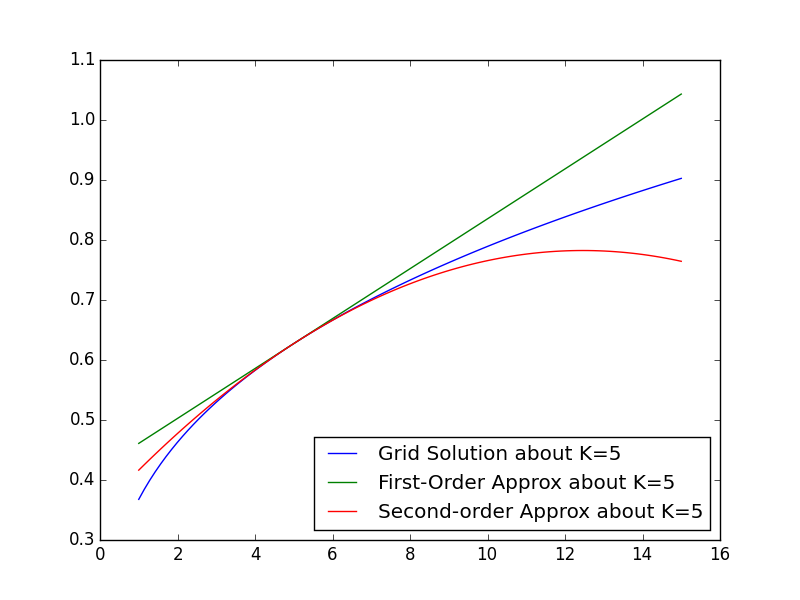
\includegraphics[scale = .75]{k5approx}
\newpage

At $k=10$, $w =0.78930333$\\
At $k=10$, $ \frac{dw}{dk} = 0.02613712$\\
At $k = 10$: $ \frac{d^2w}{dk^2} = -0.00174971$\\
Grid solution: \\
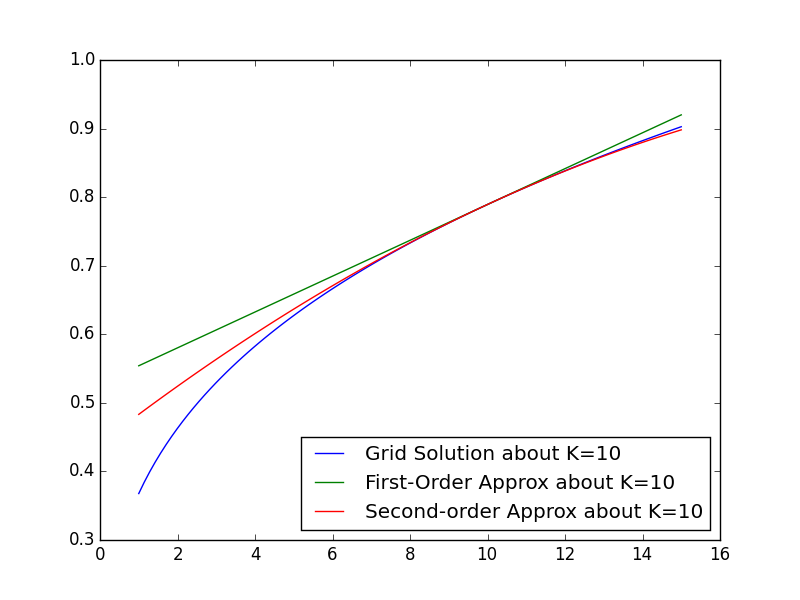
\includegraphics[scale = .75]{k10approx}

\subsection*{9.3}

$y =  47.46578754$\\
$y + \epsilon =  47.46579225$\\
$y - \epsilon = 47.46578282$\\
$y + 2\epsilon = 47.465796964$\\
$y - 2\epsilon = 47.46577811$\\
$First derivative = 0.47108525$\\
$Second derivative = 0$\\
$Third Derivative =  -10.65814104$\\

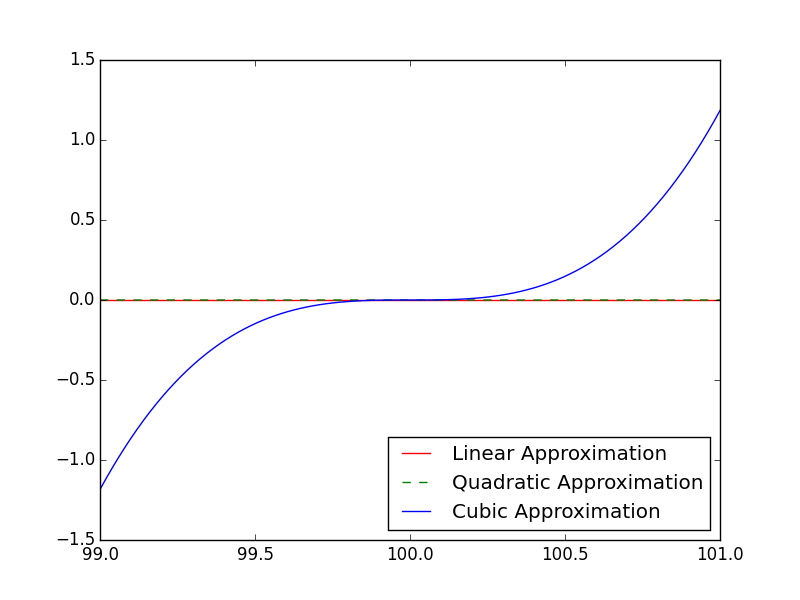
\includegraphics[scale = .75]{lqc}

\subsection*{9.4}

\[H^k(X_{t-1},Z_t,v)=H^k(\bar{X},\bar{Z},0)+\begin{bmatrix} -.0098 & .119 \end{bmatrix} \begin{bmatrix} \tilde{X}_{t-1} \\ \tilde{Z}_t \end{bmatrix}\]
\[+\frac{1}{2}\begin{bmatrix} \tilde{X}_{t-1}^T & \tilde{Z}_t^T & v \end{bmatrix} 
\begin{bmatrix}
 -.0022 & .0956 & 0 \\
 .0956 &  -.119 & 0 \\
 0 & 0 & .3202\\
\end{bmatrix}
\begin{bmatrix}
\tilde{X}_{t-1} \\
\tilde{Z}_t \\
v \\
\end{bmatrix}
\]

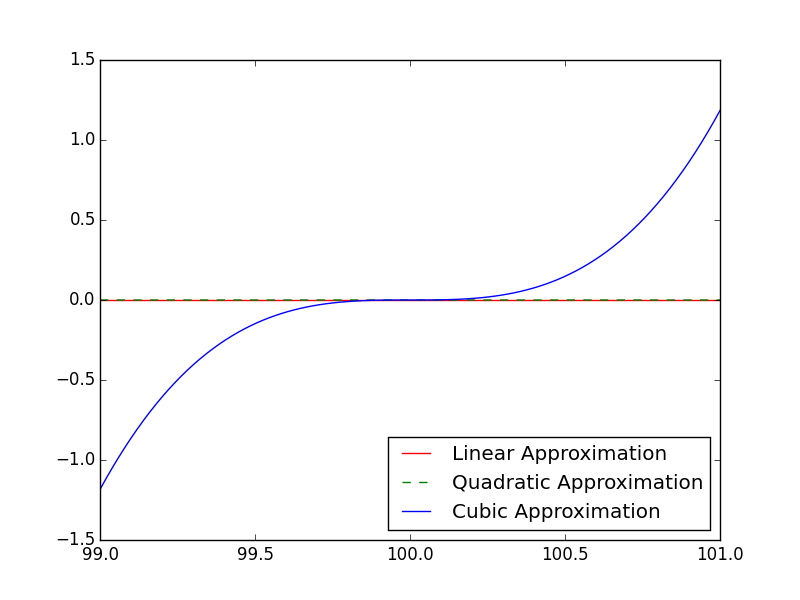
\includegraphics[scale = .75]{lqc}

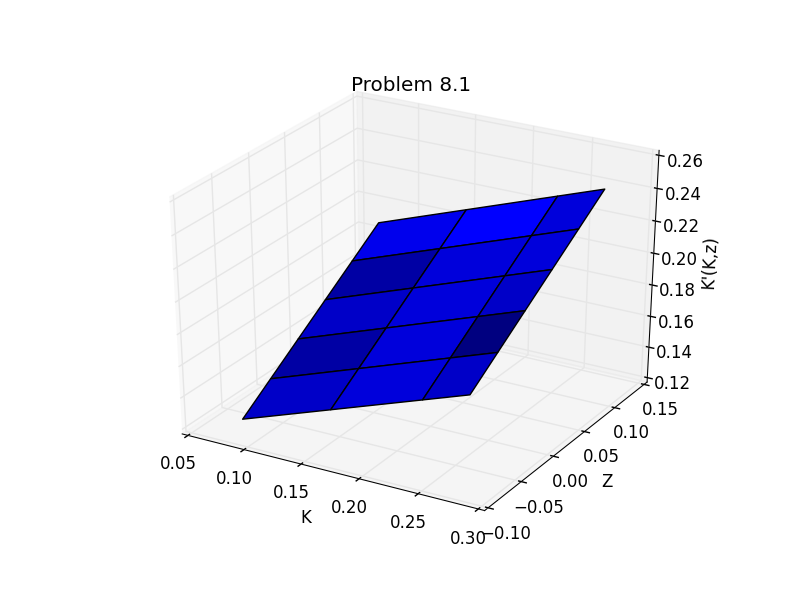
\includegraphics[scale=.75]{figure_81.png}
This graph is very similar to other models' graphs.


\end{document}
